
\chapter{Evaluation}
\label{sec:evaluation}
The employed RGB-D face detection system has already been evaluated in \cite{Fischer2010} achieving a high recall rate of 98.0\% and a precision of 98.9\%. These results can be confirmed by an experiment described in Sec. \ref{sec:evaluation:subsec:headpose}.
%In previous work the face detection, that is part of the processing pipeline has been evaluated \cite{Fischer2010}.
However, this evaluation concentrates on verifying the performance of the face recognition system especially with respect to real world influences like varying illumination, head pose and facial expressions.
%To ensure its practicability it has been evaluated regarding influences, that can occur during its application in real world scenarios.
%Those influences include variations in illumination conditions, as the camera is not in a fixed position with controlled lighting but mounted on a mobile robot.
%The minimization of the influence that pose variation of the subject's head causes is also evaluated as well as varying facial expressions.
%Additional evaluation is done on the detection people, unknown to the database.
All experiments have been carried out on publicly available databases.
We tested Support Vector Machines (SVM), K-Nearest Neighbors (KNN) and Nearest Neighbor (NN) as classifiers.
As none of these methods proved to have a great advantage over another and for the sake of simplicity, NN based on Euclidean distance has been used throughout all experiments.
The parameters for the illumination compensation algorithms used in all experiments are $\gamma$-correction, which is set to $0.2$ \cite{Tan2010}, and the number of scaled DCT coefficients, which is 5 while the scaling factor is 50.

\subsection{Databases}
\subsubsection{Extended Yale Face Database B}
The Extended Yale Face Database B \cite{Georghiades01} comprises 38 subjects with 64 illumination conditions per subject.
%Some images are corrupted and are therefore excluded from testing.
All in all there are 2414 images used in the experiments.
These images were provided already cropped to a resolution of 192 x 168 pixels and display only a manually aligned face region of the subject in frontal perspective \cite{Lee05}.

\subsubsection{AT\&T database}
%Formerly known as Olivetti Research Ltd. (ORL) database  of faces \cite{Samaria1994}
The AT\&T database contains 10 images of 40 individuals in frontal pose, thus 400 face images in total.
The subjects were unrestricted in facial expression and the 4 female and 36 male were also allowed slight variations of pose.
%The subjects were unrestricted in facial expression so the 4 female and 36 male subjects can be depicted with open or closed eyes with or without glasses.
In contrast to the Extended Yale Face Database B facial outlines are visible and the images differ slightly in scale and alignment.
The images are manually cropped to a size of 92 x 112 pixels.
%\begin{figure}[t]
%	\begin{center}
%		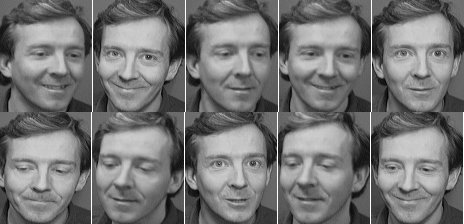
\includegraphics[width=0.9\columnwidth]{ATT_overview.jpg}
%	\end{center}
%  \caption{Typical subject from the AT\&T database of Faces.Sight slight variations in scale, pose and notable variations in facial expression are depicted}
%	\label{fig:att_overview}
%\end{figure}

\subsubsection{RGB-D Kinect Database}
The automatic head pose correction has been evaluated using data from the RGB-D Face Database \cite{Jasek2012}.
This database has been recorded using the Kinect sensor and contains color and depth data of 31 subjects recorded with 17 different head poses.
%There are 31 recorded people in 17 different head poses.
Each pose has been recorded 3 times, so altogether there are 1581 color and depth images.
To use the database for our purpose of solely analyzing the face recognition, face detection is applied beforehand and the face region in the depthmap and the color image is treated as input data for the evaluation.
%The use of the Microsoft Kinect sensor for the acquisition of this database makes it suitable for evaluation.

\subsection{Robustness to Illumination}
\label{ssec:EvalIllumination}
The implemented methods for illumination compensation have been evaluated on the extended Yale Face Database B.
According to \cite{Georghiades01}, the database was split into 5 subsets, with respect to azimuth and elevation of the light source direction with the camera axis as shown in Tab. \ref{YaleSubsets}.
\begin{table}[tb]
\caption{Subsets of the Extended Yale Face Database B}
\label{YaleSubsets}
\begin{center}
\begin{tabular}{c|c|c|c|c|c}
Subset & 1 & 2 & 3 & 4 & 5\\
\hline
Angle in [$^\circ$]  &0-10 & 10-25 & 25-50& 50-70 & $>$70\\
Number of Images & 263 & 456 &525 &456 &714\\ 
\end{tabular}
\end{center}
\end{table}
For the experiments, images with frontal and thus homogeneous illumination from  Subset 1 were used as training data.
Recognition tests were then carried out using subsets 2-5 as test data with an increasing difference in light source direction compared to the training data.
To make the impact of the illumination normalization step apparent, recognition results are reported for 
every test configuration with and without illumination compensation in Tab. \ref{tab:recognitionYale} and Fig. \ref{fig:illuminationcorrection} provides some examples of the preprocessing results.
For comprehensive comparison GammaDoG, a modified version of the illumination correction introduced by Tan et al. \cite{Tan2010} was also evaluated.
It is based on a gamma correction followed by filtering with a Difference of Gaussian filter and histogram equalization.
\begin{table}[htb]
\caption{Recognition rates on the subsets of the Yale database}
\label{tab:recognitionYale}
\begin{center}
\begin{tabular}{c|c|c|c|c}
Subset &  2 & 3 & 4 & 5 \\
\hline
%LBPH& 100\% &88\% &33.5\% &17.7\% \\
Eigenfaces& 95.83\% &51.43\% &12.06\% &3.081\% \\
Eigenfaces+LogDCT&100\% &84.38\% &70.175\% & 88.38\% \\ 
Fisherfaces& 100\% &94.0\% &39.70\%&5.74\%\\ 
Fisherfaces + HistEq &  100\% & 93.3\% & 62.7\% & 61.62\% \\ 
Fisherfaces + LogDCT & 100\% &94.3\% &85.7\% & 95.57\%\\
Fisherfaces + GammaDCT & 100\% &95.8\% &88.2\% & 96.2\%\\
Fisherfaces + GammaDoG & 100\% &99.4\% &98.0\% & 97.8\%\\
\hline
PP+LTP/DT \cite{Tan2010} & 100 \% & 100\% & 99.2 \% & 97.2 \% \\
\end{tabular}
\end{center}
\end{table}

\begin{figure}[t]
	\begin{center}
		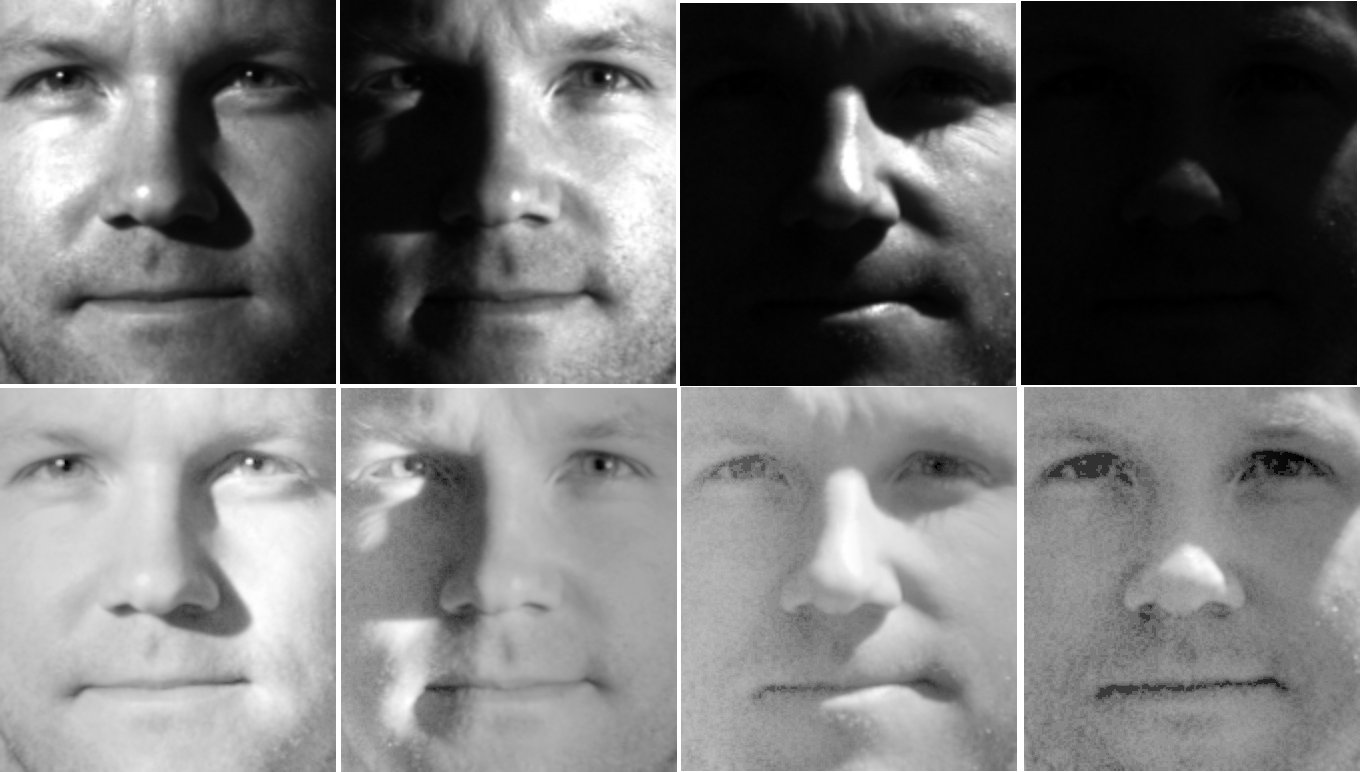
\includegraphics[width=0.9\columnwidth]{iluminationcorrection.jpg}
	\end{center}
	\caption{Illumination correction example (lower row) from Yale database. Images in upper row are taken from each subset from left to right with increasing angle between light source and camera view axis.}
	\label{fig:illuminationcorrection}
\end{figure}
As the angle of the light source increases, one can see a degradation of recognition rates of all tested algorithms, that do not include illumination compensation.
It is also apparent, that Fisherfaces handles illumination variation better than Eigenfaces, but its recognition rate is even further improved by including additional illumination normalization.  
Histogram Equalization improves recognition performance to some extent, but is outperformed by the other implemented methods.
The DCT coefficient scaling combined with a logarithm transform (LogDCT) and the DCT coefficient scaling combined with the gamma transform (GammaDCT) yield comparably good results, with a slight advantage for GammaDCT.
When Fisherfaces is combined with the GammaDoG illumination correction method the performance is furthermore improved.
Although staying slightly behind the top recognition rates of the state-of-the-art performance on the Yale Extended Database reported in \cite{Tan2010}, it is clearly shown that the improvement for Fisherfaces is significant when applying either GammaDCT, LogDCT or GammaDoG. Either of those methods can be chosen by a parameter in the provided software.
The results manifest a possible application of this recognition system in environments with lighting situations that are not covered by training data.


\subsection{Robustness to Facial Expressions}
The human face can express a variety of emotions. % among which are sadness, joy and anger.
Each one causes a notable distortion of the facial features, thus posing an additional
 challenge for the face recognition algorithm.
 To evaluate the stability of recognition performance with varying facial expression, the AT\&T database has been used.
 Tests to judge the performance under varying facial expressions included two testing strategies:
 \begin{enumerate}
   \item Leave-One-Out: 9 images per class were treated as training data and 1 image was used as test data.
   \item Leave-Half-Out: 5 images per class were treated as training data and 5 images were used as test data.
 \end{enumerate}
 Both testing strategies were carried out as tenfold cross-validation experiments, where training and test sets were chosen randomly.
 These evaluation protocols are proposed quite often in literature \cite{Naseem2010, Yang2002}.
 Recognition scores from literature are used for a comprehensive comparison of the proposed approach to state-of-the art techniques.
\begin{table}[htbp]
  \caption{Recognition rates on AT\&T database of faces}
	\label{table:att}
	\begin{center}
		\begin{tabular}{c|c|c}
		Subset & Leave-One-Out & Leave-Half-Out  \\
		\hline
		Fisherfaces& 98.75\% &95.9\% \\ 
		Fisherfaces +LogDCT& 95.8\% &94.4\% \\
		Fisherfaces +GammaDCT& 97.5\% &93.8\% \\
		Fisherfaces +GammaDoG& 87.5\% &93.8\% \\
		%FisherfacesOCV +GammaDCT&95.2\%\\ 92.9\%\\
		\hline
		LRC \cite{Naseem2010} & 98.75 \% & 93.5 \% \\
    ERE \cite{Wright2009} & 99.2 \% & 97.0 \% \\
		\end{tabular}
	\end{center}
\end{table}

The results obtained with Linear Regression (LRC) \cite{Naseem2010} are comparable to our results.
The best results are reported for Eigenface Regularization and Extraction (ERE), which achieve up to $3.2 \%$ better recognition rates than our implementation.
%The parameters of the preprocessing step were kept similar to the successful application in the examination of the performance under extreme lighting conditions.
Although all parameters of our method have been kept equal to the previous experiment a slight degradation of the recognition rates is apparent on this dataset with neutral lighting conditions for GammaDCT and to some extend for LogDCT compared to the pure Fisherfaces approach. Even more surprising, the GammaDoG normalization method causes a heavy drop in recognition rate on this database.
As GammaDCT yields more reliable results on datasets with neutral lighting and is only slightly worse under extreme conditions, it is chosen for the remaining experiments in this study.

\subsection{Robustness to Varying Head Pose}
\label{sec:evaluation:subsec:headpose}
The recognition experiments were carried out on image patches, where only the face of the person is visible.
Therefore all scenes in the database have been processed by the face detection algorithm described in section \ref{sec:methods:subsec:detection}. % after registering the color data to the depth data using the Kinect calibration data.
The face detection rates are documented in Tab. \ref{tab:EvalHeadPoseFaceDetection}, which also includes the detection rates reported by \cite{Jasek2012}.
The results are split up in results for the outer circle with viewing angles of ca. $50^\circ$ and the inner circle with about $30^\circ$ \cite{Jasek2012}.
One can see the detection rate dropping on the outer circle, but it is not influenced by varying facial expression.
It can be seen, that a $90\%$ of faces could be detected, without a single false detection.
As head pose normalization depends on finding facial features in the image, detection rates are also documented.
They are generally lower in poses on the outer circle but can cope with facial expressions very good.
\begin{table}[htbp]
  \centering
  \caption{Detection rates of faces and facial features on RGB-D DB}
  \label{tab:EvalHeadPoseFaceDetection}
  \begin{tabular}{p{2.0cm}|p{1.3cm}|p{1.3cm}|p{1.3cm}}
    pose & face detection rate& face feature detection rate & face detection rate \cite{Jasek2012}\\
    \hline
    All                  &  90.8 \%& 57.3 \%&51.7 \%\\
    Without outer circle &  95.7 \%& 66.3 \%&59.6 \%\\ 
    Only inner circle    &  95.4 \%& 63.1 \%&57.2 \%\\
    Only outer circle   &   75.3 \%& 26.1 \%&36.0 \%\\
    Facial expressions   &  95.7 \%& 95.4 \%&55.1 \%\\
    \end{tabular}
\end{table}

Images in which no face detection was possible have been excluded from the evaluation of the face recognition pipeline.
The retained cropped face images and depth maps have then been used to test the performance of the automatic head pose correction.
A cross-validation experiment has been conducted where half of the data from each subject is treated as training data and the other half as test data.
The recognition rate of $91.7\%$ is achieved on images, where faces could be detected successfully.
With respect to all images in the database $83.08\%$ of all images could be classified correctly.

In order to generate a very challenging test scenario regarding pose variation, dissimilarity in pose between training data and test data is simulated.
Therefore only images with a frontal head alignment were chosen as training images whereas the test data consisted of randomly chosen images, with variation in head pose.
10 classes have been randomly chosen, each of which provided 5 training images and 5 test images.
Please note that only images were considered, where face detection succeeded.
%The dissimilarity of the training set and the test set is documented in \ref{fig:EvalHeadPoseSetup}.
As the misalignment of faces is a major error source for the algorithm, it is tested if results can be improved by applying the automatic head pose correction described in Sec. \ref{sec:methods:pose}.
An improvement by applying both illumination normalization and head pose normalization is visible in Tab. \ref{tab:EvalPose} as well as in Fig. \ref{fig:headposecorrection}.
The overall recognition rates also indicate the difficulties for this algorithm in dealing with a big disparity of pose in training and test data.
\begin{table}
  \centering
  \caption{Recognition rates on dataset with big pose variation}
  \label{tab:EvalPose}
  \begin{tabular}{p{1.2cm}|p{1.2cm}|p{1.4cm}|p{1.4cm}}
    Method& no normalization &normalized illumination & normalized head pose \\
    \hline
    Eigenfaces & 36.2 \% & 52.7 \% & 61.8 \% \\
    Fisherfaces&41.5 \% & 56.3 \% & 68.1\% \\
  \end{tabular}
\end{table}
%\begin{figure}[htbp]
%  \begin{center}
%    \def\svgwidth{0.8\columnwidth}
%    \includesvg{../images/test}
%  \end{center}
%  \caption{\todo{describe}}
%  \label{fig:EvalHeadPoseResults}
%\end{figure}

%Results
\begin{figure}[t]
	\begin{center}
		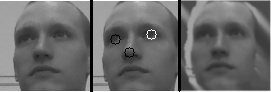
\includegraphics[width=0.9\columnwidth]{headposecorrection.jpg}
	\end{center}
	\caption{Example for the head pose correction.}
	\label{fig:headposecorrection}
\end{figure}
%discussion and interpretation

\subsection{Results in Real World Situations}
Besides the great results on common database tests we also like to emphasize the suitability of the proposed framework in real situations. To show the applicability in real applications we recorded a dozen of real situations in which some of 8 people from our lab were present. The scenes contain people working in their office, sitting at a dining table and a sofa, and show hard cases when illumination, head pose and facial expression vary. A nice overview over these scenes can be gained from the accompanying video. Fig. \ref{fig:covergirl} also displays one of those scenes. All 8 persons have been trained in all of the videos. The video also demonstrates the real time applicability of our system, which needs 250~ms for the detection step, 80~ms for head pose correction and 8~ms for the recognition with illumination normalization on a single core of a i7 2600K, 3.4 GHz.

%Record some data sets (ca. 10) with the following free parameters:
%- ground truth faces learned only in one single situation with certain conditions (conditions may be different for different people)
%- numerous people (ca. 10)
%- different head orientations
%- light switched on/off
%- indoor/outdoor
%- facial expressions
%- moving people
%- realistic situations (i.e. cob lab: kitchen, sofa, table, ...)
%- unknown people
%
%Success is judged on the accumulated tracking results, i.e. have the people been labeled correctly most of the time.
%
%- runtime (rec+illum: 8ms,  rec+illum+head: 80ms, face det. 250ms) single core i7 2600K, 3.4 GHz, 16 GB RAM

\subsection{Recognizing Unknown People}
In order to judge the practicability of the threshold selection mentioned described in Sec. \ref{ssec:IdentificationUnknown}, the recognition performance on two databases was examined regarding classification.
For the experiment, the database was divided into two subsets. Half of the classes were not included in the training data, thus keeping the excluded people unknown.
Of the remaining subset, half of the images of each class was used as training data.
The test data consists consequently of images of both unknown and known individuals.
This experiment was carried out on the Extended Yale Database B and the AT\&T database.
The division into subsets is done according to table \ref{tab:EvalUnknownDivision}.

\begin{table}[htbp]
  \centering
  \caption{Subdivision of databases that were used for evaluation identification of unknown people}
  \label{tab:EvalUnknownDivision}
  \begin{tabular}{c|p{0.8cm}|p{0.8cm}|p{0.8cm}|p{0.8cm}|p{0.8cm}|p{0.8cm}}
    Database&\multicolumn{3}{|c|}{Training Set}&\multicolumn{3}{|c}{Test Set}\\
    \hline
    &images & classes known & classes unknown& images & samples known & samples unknown\\
    \hline
    AT\&T &100 & 20 &20 & 300 & 100 & 200\\
    Yale & 605 & 19 &21 & 1809 & 603 &1206\\
  \end{tabular}
\end{table}

The classification is only considered correct when either an unknown person is classified unknown, or a known person is assigned to the right class.
Training data and test data was chosen randomly and recognition rates were verified using tenfold cross-validation.
Results can be seen in Tab. \ref{tab:EvalUnknownThreshold}.

%\begin{figure}[htbp]
%  \begin{center}
%    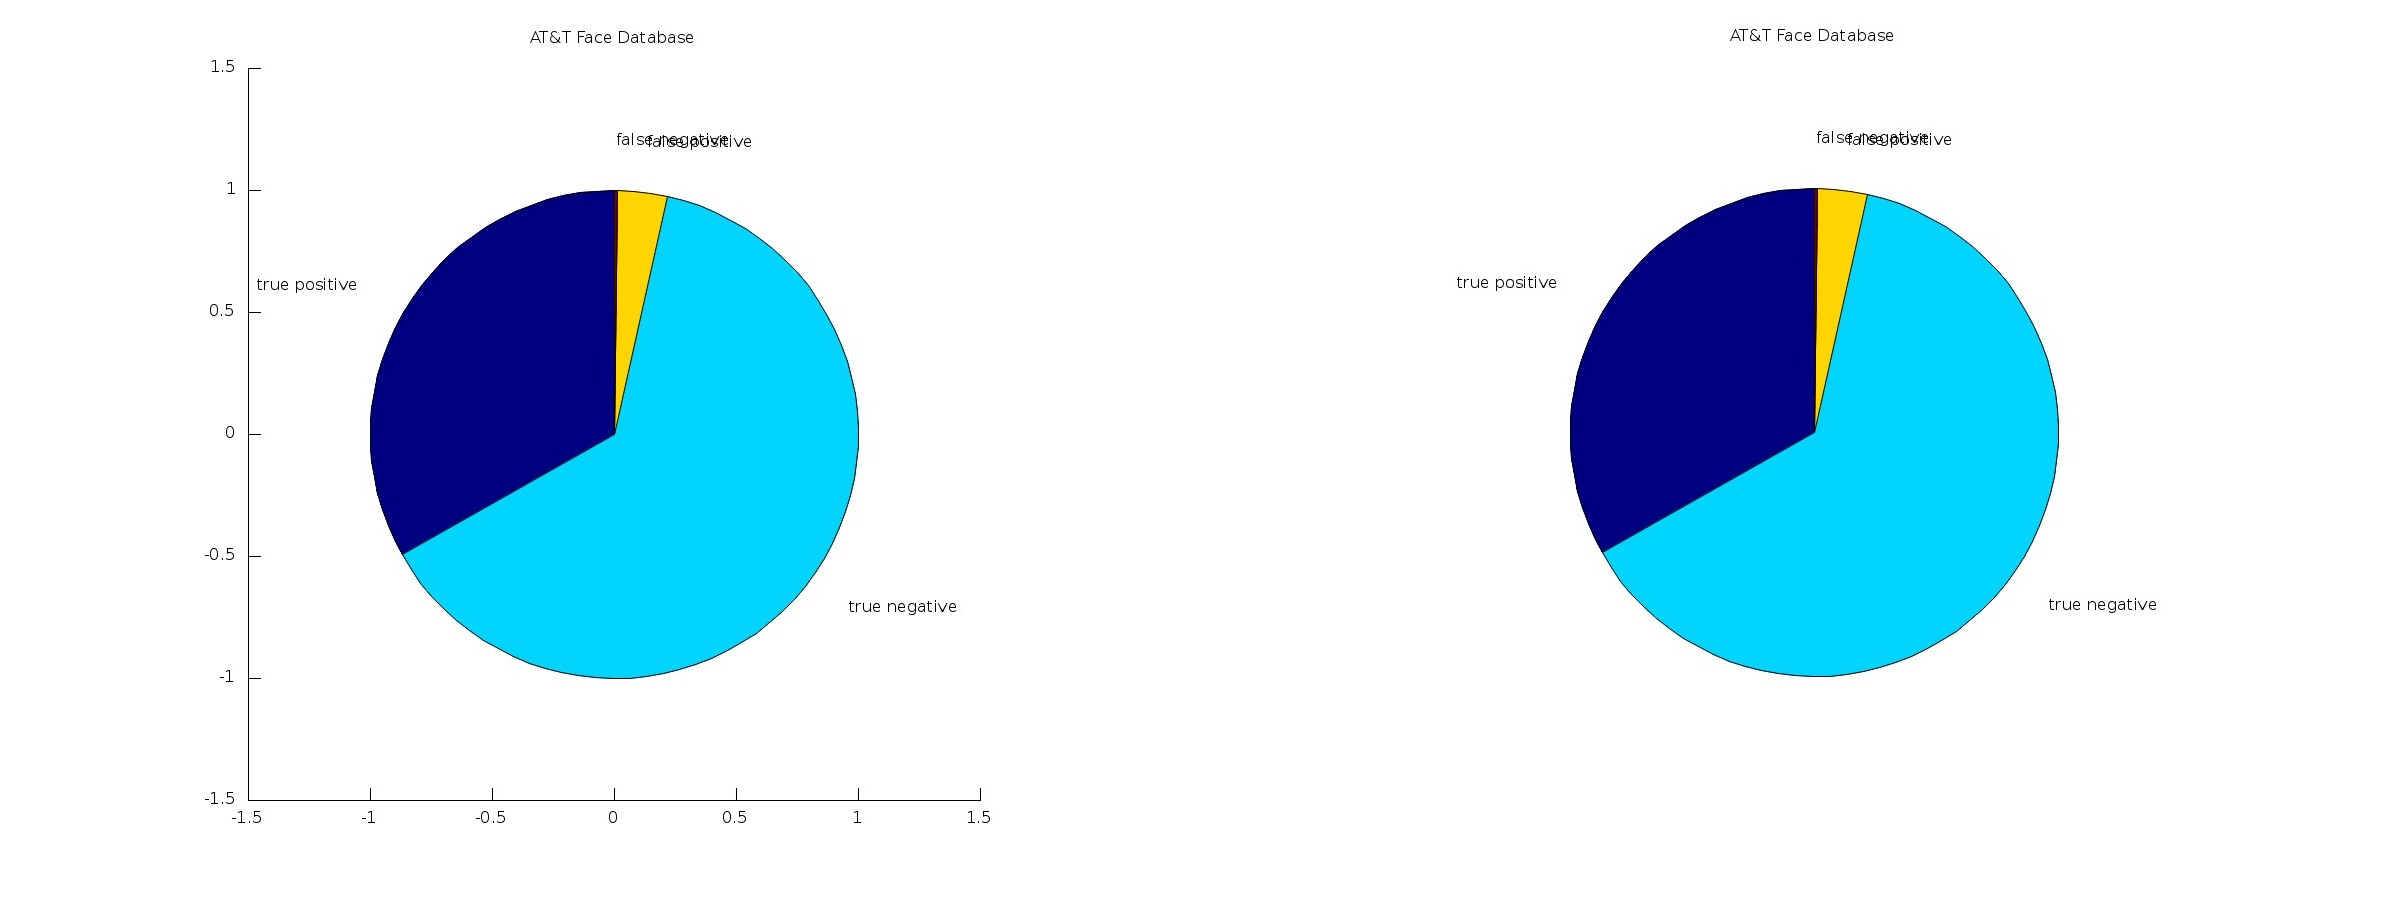
\includegraphics[width=0.8\columnwidth]{PieUnknownATTYALE.jpg}
%  \end{center}
%  \caption{\todo{describe+minipage + table + intuitive colors in grayscale}}
%  \label{fig:EvalUnknownPie}
%\end{figure}

\begin{table}[htbp]
  \centering
  \caption{Results for recognition of unknown people}
  \label{tab:EvalUnknownThreshold}
  \begin{tabular}{l|p{0.8cm}|p{0.8cm}|p{0.8cm}|p{0.8cm}|p{0.9cm}}
    Scenario & True \newline Positive & False \newline Positive & False \newline Negative & True \newline Negative  &   Recognition rate\\
    \hline
    AT\&T &82.4 \%  & 17.6\% & 2.4\% & 97.6\%& 92.5 \% \\
    Yale & 99.4 \%& 0.5 \%& 4.93\% & 94.9\% & 96.5 \% \\
  \end{tabular}
\end{table}
The results on the tested databases show, that the dynamic threshold application has the potential of distinguishing between known people and unknown people.
Although the size of the training data sets is different for both databases, our solution still achieves a high overall recognition rate of over $90 \%$ in both cases.

%\subsection{Single Color Camera}
